%% authors
%\author{Paul Deveau\\Institut Curie\\PSL University\\Univ. Paris-Sud\\INSERM U830\\INSERM U900\\Mines-ParisTech \And 
%        Emmanuel Barillot\\Institut Curie\\PSL University\\INSERM U900\\Mines-ParisTech \And 
%        Valentina Boeva\\Institut Curie\\PSL University\\INSERM U900\\Mines-ParisTech\\Institut Cochin\\INSERM U1016\\CNRS UMR 8104\\Paris Descartes University UMR-S1016 \AND 
%        Andrei Zinovyev\\Institut Curie\\PSL University\\INSERM U900\\Mines-ParisTech \And
%        Eric Bonnet\\Institut Curie\\PSL University\\INSERM U900\\Mines-ParisTech}
%\title{Calculating Biological Module Enrichment or Depletion and Visualizing Data on Large-scale Molecular Maps with the \R packages \pkg{ACSNMineR} and \pkg{RNaviCell}}

%% for pretty printing and a nice hypersummary also set:
\author{by Paul Deveau, Emmanuel Barillot, Valentina Boeva, Andrei Zinovyev and Eric Bonnet} %% comma-separated
\title{Calculating Biological Module Enrichment or Depletion and Visualizing Data on Large-scale Molecular Maps with \pkg{ACSNMineR} and \pkg{RNaviCell} packages} %% without formatting
%\Shorttitle{Module Enrichment and Data Visualization with ACSNMineR and RNaviCell} %% a short title (if necessary)
\maketitle
%% publication information


%% an abstract and keywords
\abstract{
Biological pathways or modules represent sets of interactions or functional relationships occurring at the molecular level in living cells. A large body of knowledge on pathways is organized in public databases such as the KEGG, Reactome, or in more specialized repositories, the Atlas of Cancer Signaling Network (ACSN) being an example. All these open biological databases facilitate analyses, improving our understanding of cellular systems. We hereby describe \CRANpkg{ACSNMineR} for calculation of enrichment or depletion of lists of genes of interest in biological pathways. \pkg{ACSNMineR} integrates ACSN molecular pathways, but can use any molecular pathway encoded as a GMT file, for instance sets of genes available in the Molecular Signatures Database (MSigDB). We also present \CRANpkg{RNaviCell}, that can be used in conjunction with \pkg{ACSNMineR} to visualize different data types on web-based, interactive ACSN maps. We illustrate the functionalities of the two packages with biological data taken from large-scale cancer datasets.  


}
%\Keywords{biological module, biological pathway, enrichment, depletion, cancer, maps, molecular networks, molecular pathways, \proglang{R}}
%\Plainkeywords{biological module, biological pathway, enrichment, depletion, cancer, maps, molecular networks, molecular pathways, R} %% without formatting





%% include your article here, just as usual
%% Note that you should use the \pkg{}, \proglang{} and \code{} commands.

\section[Introduction]{Introduction}
Biological pathways and networks comprise sets of interactions or functional
relationships, occurring at the molecular level in living cells
\citep{adriaens2008public, barillot2012computational}.  A large body of
knowledge on cellular biochemistry is organized in publicly available
repositories such as the KEGG database \citep{kanehisa2011kegg}, Reactome
\citep{croft2014reactome} and MINT \citep{zanzoni2002mint}. All these
biological databases facilitate a large spectrum of analyses, improving our
understanding of cellular systems. For instance, it is a very common practice
to cross the output of high-throughput experiments, such as mRNA or protein
expression levels, with curated biological pathways in order to visualize the
changes, analyze their impact on a network and formulate new hypotheses about
biological processes. Many biologists and computational biologists establish
list of genes of interest (e.g. a list of genes that are differentially
expressed between two conditions, such as normal vs disease) and then evaluate
if known biological pathways have significant overlap with this list of genes. 

We have recently released the Atlas of Cancer Signaling Network (ACSN), a
web-based database which describes signaling and regulatory molecular processes
that occur in a healthy mammalian cell but that are frequently deregulated
during cancerogenesis \citep{kuperstein2015atlas}.  The ACSN atlas aims to
be a comprehensive description of cancer-related mechanisms retrieved from the
most recent literature. The web interface for ACSN is using the NaviCell
technology, a software framework dedicated to web-based visualization and
navigation for biological pathway maps \citep{kuperstein2013navicell}. This
environment is providing an easy navigation of maps through the use of the
Google Maps JavaScript library, a community interface with a web blog system,
and a comprehensive module for visualization and analysis of high-throughput
data \citep{bonnet2015navicell}.


In this article, we describe two packages related to ACSN analysis and
data visualization. The package \CRANpkg{ACSNMineR} is designed for the calculation of
gene enrichment and depletion in ACSN maps (or any user-defined gene set via
the import function), while \CRANpkg{RNaviCell} is dedicated to data visualization
on ACSN maps. Both packages are available on the Comprehensive R Archive
Network (\url{https://cran.r-project.org/web/packages/ACSNMineR/} and
\url{https://cran.r-project.org/web/packages/RNaviCell/}), and on the GitHub
repository (\url{https://github.com/sysbio-curie/ACSNMineR} and
\url{https://github.com/sysbio-curie/RNaviCell}). For the remainder of this
article, we describe the organization of each package and illustrate their
capacities with several concrete examples demonstrating their capabilities. 

\section[Packages organization]{Packages organization}

\subsection{ACSNMineR}
Currently, ACSN maps cover signaling pathways involved in DNA repair, cell
cycle, cell survival, cell death, epithelial-to-mesenchymal transition (EMT) and
cell motility. Each of these large-scale molecular maps is decomposed in a number
of functional modules. The maps themselves are merged into a global ACSN map.
Thus the information included in ACSN is organized in three hierarchical levels:
a global map, five individual maps, and several functional modules. Each
ACSN map covers hundreds of molecular players, biochemical reactions and causal
relationships between the molecular players and cellular phenotypes.  ACSN
represents a large-scale biochemical reaction network of 4,826 reactions
involving 2,371 proteins (as of today), and is continuously updated and expanded.  We have
included the three hierarchical levels in the \pkg{ACSNMineR} package, in order
to be able to calculate enrichments at all three levels. The calculations are
made by counting the number of occurences of gene symbols (HUGO gene names) from
a given list of genes of interest in all ACSN maps and modules. Table
\ref{tab:table1} is detailling the number of gene symbols contained in all the ACSN
maps.


\begin{table}[h!]
 \centering
  \caption{ACSN maps included in the \pkg{ACSNMineR} package. Map: map name,
  Total: total number of gene symbols (HUGO) used to construct the map, Nb
  mod.: number of modules, Min: mimimum number of gene symbols in the modules,
  Max: maximum number of gene symbols in the modules, Mean: average number of
  gene sybols per module. N.B.: one gene symbol may be present in several
  modules of the map.} \label{tab:table1}
  \begin{tabular}{l c c c c c}
    \toprule
    Map & Total & Nb mod. & Min & Max & Mean\\
    \midrule
  ACSN global & 2243 & 63 & 2 &629& 83\\
  Survival  &1053&5  &208 &431 &328\\
  Apoptosis & 667&7 & 19& 382& 136\\
  EMT \& Cell motility &634 &9  &18 &629 &136\\
  DNA repair &345&21  &3 &171  &45\\
  Cell cycle &250&25  &2 &130  &19\\
  \bottomrule

  \end{tabular}

\end{table}


The statistical significance of the counts in the modules is assessed by using
either the Fisher exact test \citep{fisher1922interpretation,
fisher1934statistical} or the hypergeometric test, which are equivalent for this
purpose \citep{rivals2007enrichment}.

The current ACSN maps are included in the \pkg{ACSNMineR} package, as a list of character matrices.

\begin{example}
> length(ACSN_maps)
[1] 6
> names(ACSN_maps)
[1] "Apoptosis"    "CellCycle"    "DNA_repair"   "EMT_motility" "Master" 
[6] "Survival"    
\end{example}

For each matrix, rows represent a module, with the name of the module in the
first column, followed by a description of the module (optional), and then
followed by all the gene symbols of the module. The maps will be updated
according to every ACSN major release.

The main function of the \pkg{ACSNMineR} package is the \code{enrichment}
function, which is calculating over-representation or depletion of genes in the
ACSN maps and modules. We have included a small list of 12 Cell Cycle related
genes in the package, named \code{genes\_test} that can be used to test the main
enrichment function and to get familiar with its different options.

\begin{example}
> genes_test
 [1] "ATM"     "ATR"     "CHEK2"   "CREBBP"  "TFDP1"   "E2F1"    "EP300"  
 [8] "HDAC1"   "KAT2B"   "GTF2H1"  "GTF2H2"  "GTF2H2B"
\end{example}

The example shown below is the simplest command that can be done to test a gene
list for over-representation on the six included ACSN maps. With the list of 12
genes mentionned above and a default p-value cutoff of $0.05$, we have a set of
36 maps or modules that are significantly enriched. The results are structured
as a data frame with nine columns displaying the module name, the module size,
the number of genes from the list in the module, the names of the genes that are
present in the module, the size of the reference universe, the number of genes
from the list that are present in the universe, the raw p-value, the p-value
corrected for multiple testing and the type of test performed. The module field
in the results data frame indicate the map name and the module name separated by
a column character. If a complete map is significantly enriched or depleted,
then only the map name is shown, without any module or column character. For
instance, the third line of the results object below concern the E2F1 module of
the CellCycle map. 


\begin{example}
> library(ACSNMineR)
> results <- enrichment(genes_test)
> dim(results)
[1] 8  9
> results[3,]
            module module_size nb_genes_in_module
V161 CellCycle:E2F1          19                 12
                                                             genes_in_module
V161 ATM ATR CHEK2 CREBBP TFDP1 E2F1 EP300 HDAC1 KAT2B GTF2H1 GTF2H2 GTF2H2B
     universe_size nb_genes_in_universe      p.value p.value.corrected    test
V161          2237                   12 3.735018e-21      2.353061e-19 greater
\end{example}


%    enrichment(Genes = NULL, maps = ACSNMineR::ACSN_maps,
%       correction_multitest = "BH", statistical_test = "fisher",
%       min_module_size = 5, universe = "map_defined", threshold = 0.05,
%       alternative = "greater")

The \code{enrichment} function can take up to eight arguments: the gene list (as
a character vector), the list of maps that will be used to calculate enrichment
or depletion, the type of statistical test (either the Fisher exact test or the
hypergeometric test), the module minimal size for which the calculations will be
done, the universe, the p-value threshold and the alternative ("greater" for
calculating over-representation, "less" for depletion and "both" for both
tests).

Only the gene list is mandatory to call the \code{enrichment} function, all the
other arguments have default values.  The \code{maps} argument can either be a
dataframe imported from a gmt file with the \code{format\_from\_gmt} function or
a list of dataframes generated by the same procedure. By default, the function
uses the ACSN maps previously described.  The correction for multiple testing
is set by default to use the method of Benjamini \& Hochberg, but can be
changed to any of the usual correction methods (Bonferroni, Holm, Hochberg,
Holm, or Benjamini \& Yekutieli \citep{Benjamini2003FDR}), or even disabled .
The minimal module size represents the smallest size value of a module that
will be used to compute enrichment or depletion. This is meant to remove
results of low significance for module of small size.  The universe in which
the computation is made by default is defined by all the gene symbols contained
in the maps. All the genes that were given as input and that are not present on
the maps will be discarded. To keep all genes, the user can change the universe
to \code{HUGO}, and in that case, the complete list of HUGO gene symbols will
be used as the reference ($>$ 39,000 genes). The threshold corresponds to the
maximal value of the corrected p-value (unless the user chose not to correct
for multiple testing) that will be displayed in the result table.


%multisample_enrichment<-function(Genes_by_sample=NULL,
%                                 maps = ACSNMineR::ACSN_maps, 
%                                 correction_multitest = "BH",
%                                 statistical_test = "fisher",
%                                 min_module_size = 5,
%                                 universe = "map_defined",
%                                 threshold = 0.05,
%                                 cohort_threshold = TRUE,
%                                 alternative = "greater"){


It may be of interest to compare enrichment of pathways in different cohorts or
experiments. For example, enrichment of highly expressed pathways can reveal
differences between two cancer types or two cell lines.  To facilitate such
comparisons, \pkg{ACSNMineR} provides a \code{multisample\_enrichment} function.
It relies on the \code{enrichment} function but takes a list of character
vector genes. The name of each element of the list will be assumed to be the
name of the sample for further analysis.  Most of the arguments given to
\code{multisample\_enrichment} are the same as the ones passed to
\code{enrichment}. However, the \code{cohort\_threshold} is designed to filter
out modules which would not pass the significance threshold in all samples.   

%represent_enrichment<-function(enrichment, plot = "heatmap" , scale = "log", 
%                               low = "steelblue" , high ="white",
%                              nrow = 1,sample_name = "Sample",
%                               na.value = "grey"){

Finally, to facilitate visualization of results, \pkg{ACSNMineR} integrates a
representation function based on \CRANpkg{ggplot2} syntax \citep{ggplot2}. It
allows representation of results from \code{enrichment} or
\code{multisample\_enrichment} with a limited number of parameters. Two types of
display are available: heat-map tiles or bars. For multiple samples using a
barplot representation, the number of rows used can be provided, otherwise all
plots will be on the same row. For the heatmap, the color of the
non-significant modules, and boundaries of the gradient for significant values
can also be tuned.

We previously computed the p-value of the \code{genes\_test} list with default
parameters. The number of modules which have a p-value below 0.05 was 36, that
can be compared to the 49 obtained without correction with the simple command
shown below (some of the results are displayed in table \ref{tab:table2}).


\begin{example}
enrichment(genes_test,correction_multitest = FALSE)
\end{example}


\begin{widetable}[h!]
  \centering
  \caption{Overview of the results from enrichment analysis without correction.
  Module : name of the module. Mod. size: size of the module. Genes in module:
  genes from input which are found in the module. p-value: uncorrected p-value.
  Test : null hypothesis used, greater is synonym of enrichment.}
  \label{tab:table2}

  \begin{tabular}{l c c c c}
	\toprule
Module & Mod. size & Genes in module & p-value & Test\\
	\midrule
CellCycle & 242 & ATM ATR CHEK2   & 5.36e-07 & greater \\
          &   &  CREBBP KAT2B TFDP1   &          &         \\
          &   &  E2F1 EP300 HDAC1    &          &         \\
          &	  & GTF2H1 GTF2H2 GTF2H2B &	& \\
CellCycle: APOPTOSIS ENTRY & 10 & ATM ATR CHEK2 E2F1 & 3.49e-07 & greater \\
CellCycle: CYCLINB			& 7  & ATM 				  & 3.98e-02 & greater \\



	\bottomrule

	\end{tabular}
\end{widetable}

We can now plot the first six rows of the results obtained for corrected and
uncorrected fisher test with heatmap format (Figure~\ref{fig:heatm}) or barplot
(Figure~\ref{fig:barp}) with the following commands:

\begin{example}
# heatmap

represent_enrichment(enrichment = list(Corrected = results[1:6,], 
Uncorrected = results_uncorrected[1:6,]),
                                plot = "heatmap", scale = "reverselog", 
                                low = "steelblue" , high ="white", na.value = "grey")

# barplot 

 represent_enrichment(enrichment = list(Corrected = results[1:6,], 
                             Uncorrected = results_uncorrected[1:6,]),
                               plot = "heatmap", scale = "reverselog", 
                               nrow = 1)
\end{example}

\begin{figure}[h!]
	\centering
    \caption{Representation of the enriched modules (first six rows for each setting), with
    either Bonferroni correction or no correction. Grey tiles means that the
    data is not available for this module in this sample. P-values of low
    significance are in white, whereas p-values of high significance are
    represented in blue.}
    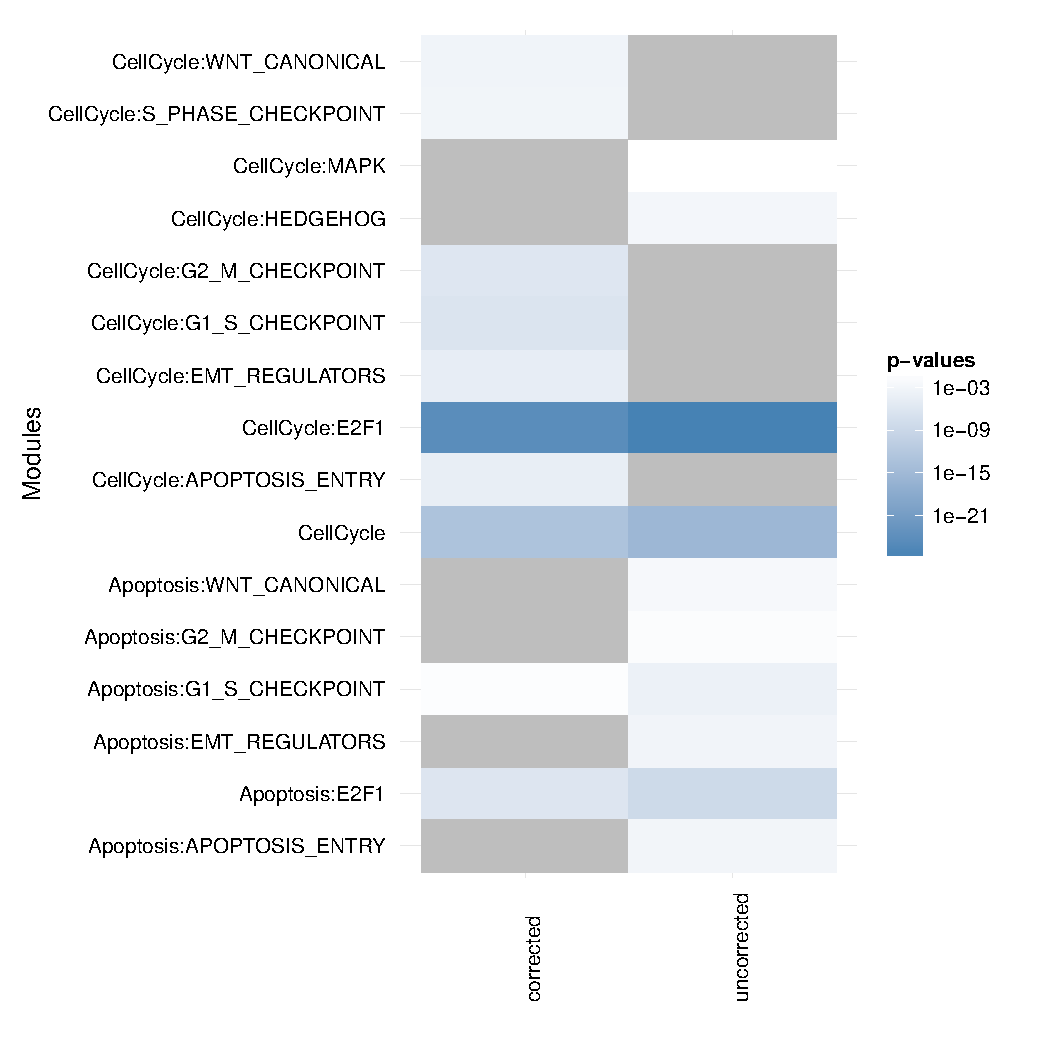
\includegraphics[width=0.8\textwidth]{figures/comparison_corrected_unc.pdf}
    \label{fig:heatm}

\end{figure}


\begin{figure}[h!]
	\centering
	\caption{Representation of the enriched modules (first six rows for each setting), with either Bonferroni correction (left) or no correction (right). The modules are on the X axis and the p-values are on the Y axis.  }
	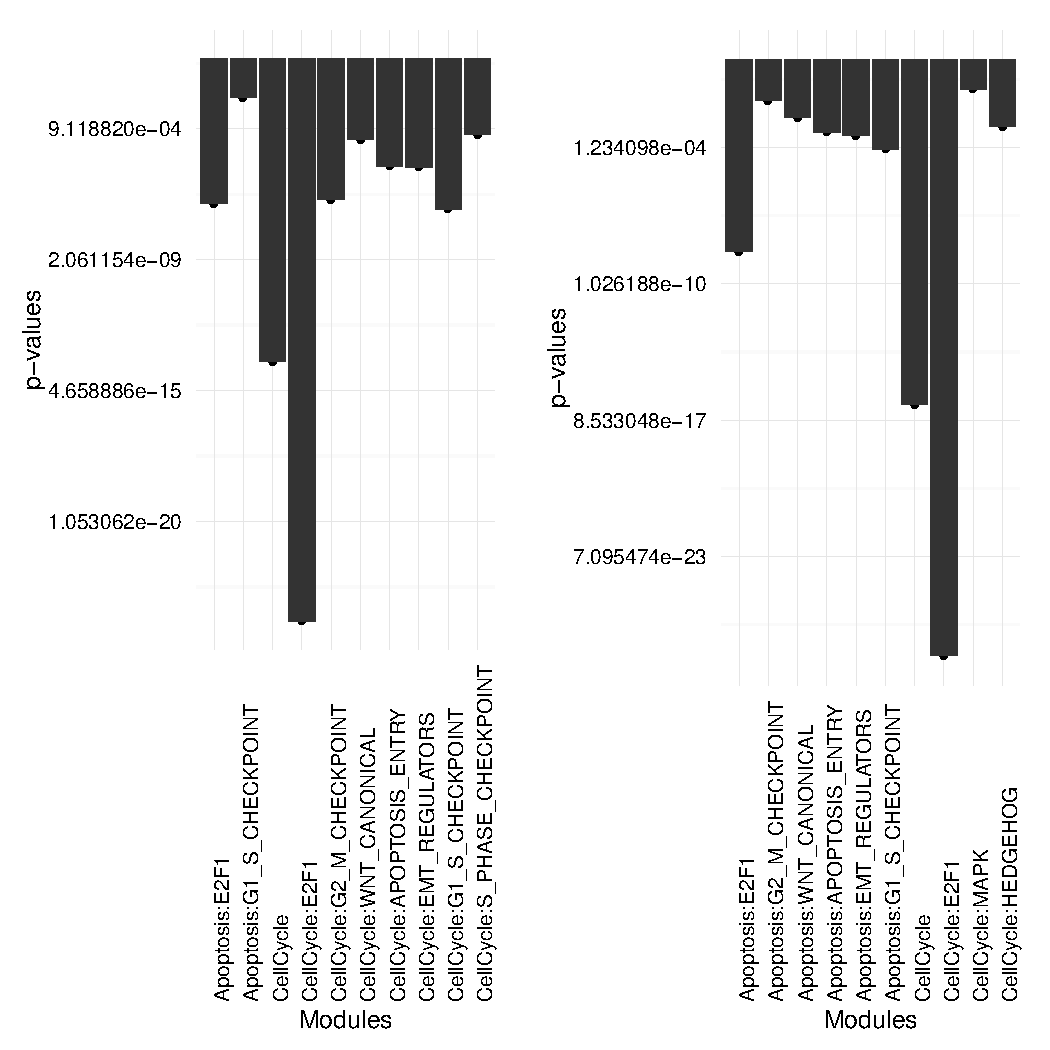
\includegraphics[width=\textwidth]{figures/comparison_corrected_unc_bars.pdf}
	\label{fig:barp}

\end{figure}




\subsection{RNaviCell}

The NaviCell Web Service provides a server mode, which allows automating
visualization tasks and retrieving data from molecular maps via RESTful
(standard http/https) calls. Bindings to different programming languages are
provided in order to facilitate the development of data visualization workflows and
third-party applications \citep{bonnet2015navicell}. RNaviCell is the R binding
to the NaviCell Web Service. It is implemented as a standard R package, using
the R object-oriented framework known as Reference Classes \citep{hwR5}. Most
of the work done by the user using graphical point-and-click operations on the
NaviCell web interface are encoded as functions in the library encapsulating
http calls to the server with appropriate parameters and data. Calls to the
NaviCell server are performed using the library RCurl \citep{rcurl2015}, while
data encoding/decoding in JSON format is performed with the RJSONIO library
\citep{rjsonio2014}.

Once the RNaviCell library is installed and loaded, the first step is to create
a NaviCell object and launch the browser session. This will automatically create
a unique session ID with the NaviCell server. Once the session is established,
various functions can be called to send data to the web session, set graphical
options, visualize data on a map or get data from the map. There are 125
functions available in the current version of RNaviCell. All of them are
described with their different options in the RNaviCell documentation, and we
provide a tutorial on the GitHub repository wiki
(\url{https://github.com/sysbio-curie/RNaviCell/wiki/Tutorial}).  

In the simple example detailed below, we create a NaviCell session, then load
an expression data set from a local (tab-delimited) file. The data represent
gene expression measured in a prostate cancer cell line resistant to hormonal
treatment (agressive), and is taken from the Cell Line Encyclopedia project
\citep{barretina2012cancer}. We visualize the data values on the Cell Cycle map
(the default map), using heat maps. With this visualization mode, gene
expression values are represented as a color gradient (green to red) in
squares positioned next to the entities where the gene has been mapped (Figure~\ref{fig:du145}).      


\begin{figure}[!ht]
  \caption{Gene expression values from a prostate cancer cell line visualized
on the cell cycle map as heat map plots. The figure is a screenshot of the
NaviCell map browser, with the map set at the top (the less detailed) zoom
level. The essential phases of the cell cycle are indicated on the map
(G1/S/G2/M). Note that on the web browser the map is interactive and the user
can zoom in and out, change the graphical parameters, import additional data
and perform functional analysis.  } 
\centering
  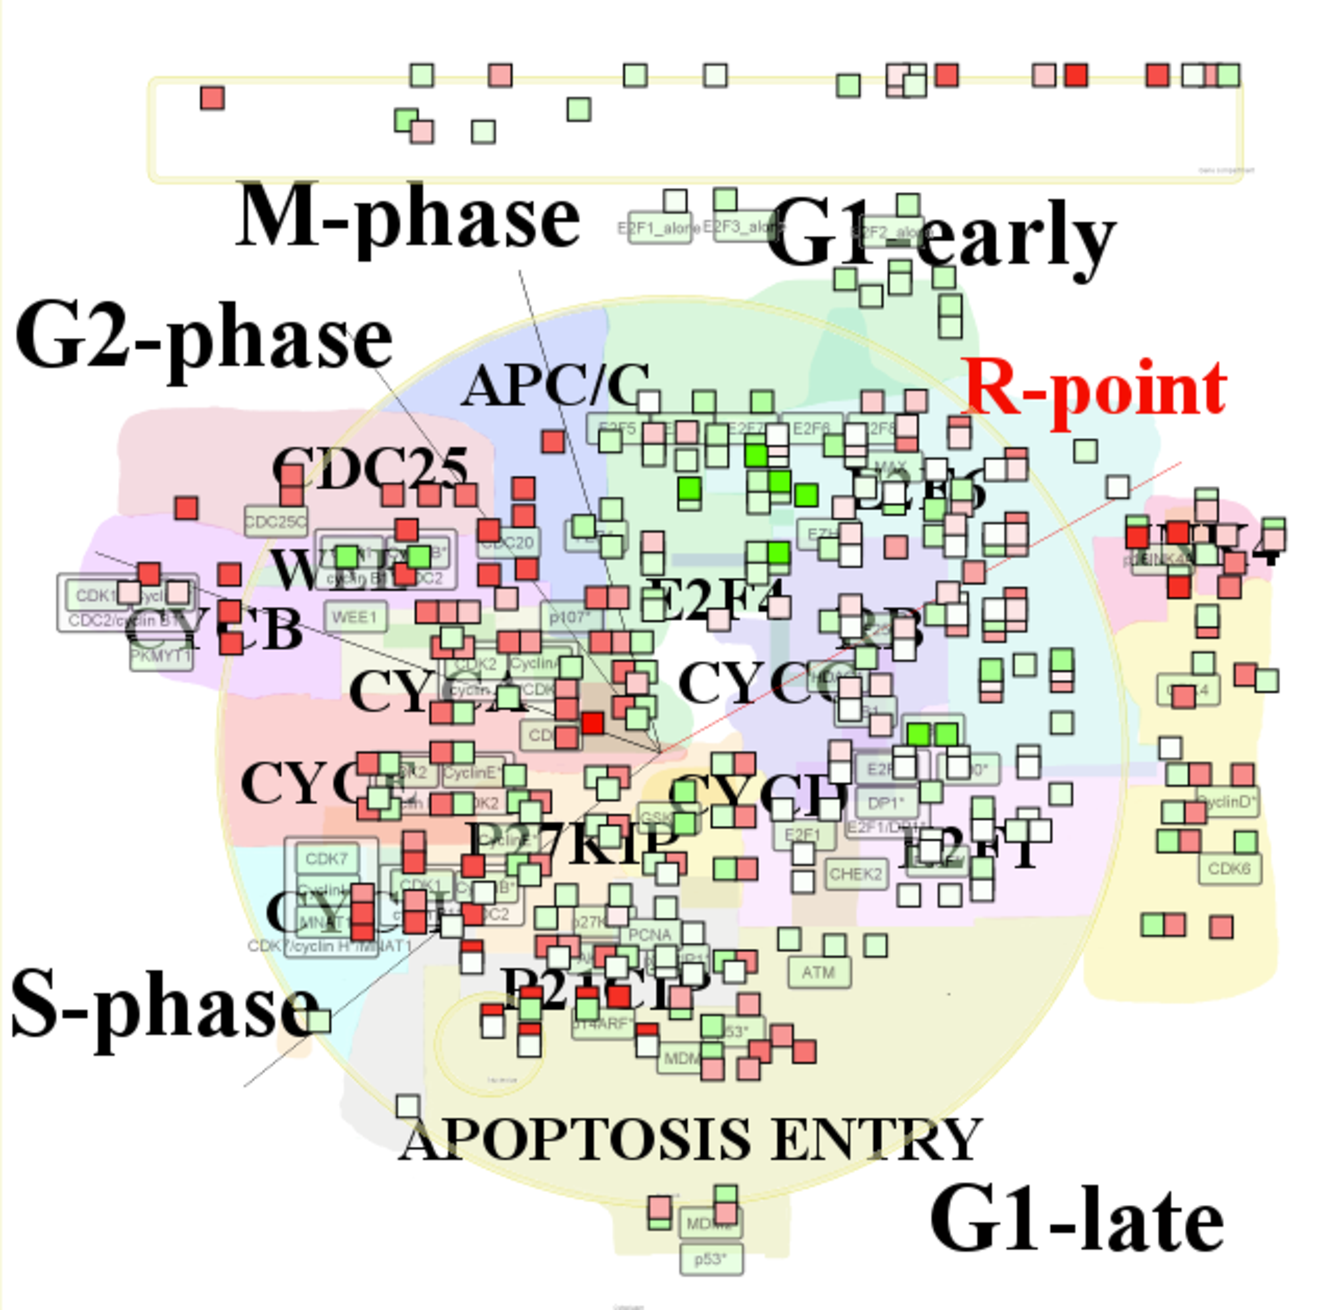
\includegraphics[width=0.8\textwidth]{figures/heatmap.pdf}
  \label{fig:du145}
\end{figure}



\begin{example}
# a short RNaviCell script example

# load RNaviCell library

library(RNaviCell)

# create a NaviCell object and launch a server session
# this will automatically open a browser on the client 

navicell <- NaviCell()
navicell$launchBrowser()

# import a gene expression matrix and 
# send the data to the NaviCell server
# NB: the data_matrix object is a regular R matrix

data_matrix <- navicell$readDatatable('DU145_data.txt')
navicell$importDatatable("mRNA expression data", "DU145", data_matrix)

# set data set and sample for heat map representation

navicell$heatmapEditorSelectSample('0','data')
navicell$heatmapEditorSelectDatatable('0','DU145')
navicell$heatmapEditorApply()

\end{example}

\section[Case studies]{Case studies}

\subsection{Analysis of breast cancer expression data}
In a study published in 2008, Schmidt and colleagues analyzed gene expression
patterns of 200 breast cancer patients not treated by systemic therapy after
surgery using discovery approach to reveal additional prognostic motifs
\citep{schmidt2008humoral}. Estrogen receptor (ER) expression and proliferative
activity of breast carcinomas are well-known and described prognostic markers.
Patients with ER-positive carcinomas have a better prognosis than those with
ER-negative carcinomas, and rapidly proliferating carcinomas have an adverse
prognosis. Knowledge about the molecular mechanisms involved in the
processes of estrogen-dependent tumor growth and proliferative activity has led
to the successful development of therapeutic concepts, such as  antiendocrine and
cytotoxic chemotherapy. 

The dataset corresponding to this study is available as a Bioconductor package.
The code shown below is creating a list of differentially expressed genes
between ER positive and ER negative samples, and calculates the enrichment in
ACSN maps from this list of genes. As seen in Table \ref{tab:table_mainz},
there is one map (Cell Cycle) and six modules (belonging to the Cell Cycle, DNA
repair and EMT motility maps) enriched. 

\begin{example}
# load all necessary packages
library(breastCancerMAINZ)
library(Biobase)
library(limma)
library(ACSNMineR)
library(hgu133a.db)
library(RNaviCell)

# load data and extract expression and phenotype data 
data(mainz)
eset <- exprs(mainz)
pdat <- pData(mainz)

# Create list of genes differentially expressed between ER positive and 
# ER negative samples using moderated t-test statistics 
design <- model.matrix(~factor(pdat$er == '1'))
lmFit(eset, design) -> fit
eBayes(fit) -> ebayes
toptable(ebayes, coef=2,n=25000) -> tt
which(tt$adj < 0.05) -> selection
rownames(tt[selection,]) -> probe_list
mget(probe_list, env=hgu133aSYMBOL) -> symbol_list
symbol_list <- as.character(symbol_list)

# calculate enrichment in ACSN maps 

enrichment(symbol_list) -> results

dim(results)
[1] 8 9
\end{example}

\begin{table}[h!]
  \centering
  \caption{ACSN maps enrichment for genes differentially expressed between ER
positive and ER negative samples in breast cancer.  Module : name of the
module. Mod. size: size of the module. Nb genes: number of genes from input
which are found in the module. pval: raw p-value. Cor. pval: corrected p-value.}
\label{tab:table_mainz}

\begin{tabular}{l c c c c}
\toprule
Module & Mod. size & Nb genes & pval & Cor. pval\\
\midrule
  Apoptosis:AKT\_MTOR & 79 & 47 & 0.00043 & 0.0068 \\ 
  CellCycle:E2F2\_TARGETS & 35 & 22 & 0.0055 & 0.043 \\ 
  CellCycle:E2F3\_TARGETS & 51 & 31 & 0.0023 & 0.025 \\ 
  CellCycle:E2F4\_TARGETS & 100 & 60 & $5.8 \times 10^{-5}$ & 0.0037 \\ 
  DNA\_repair & 346 & 172 & 0.00038 & 0.0068 \\ 
  DNA\_repair:CELL\_CYCLE & 82 & 49 & 0.00029 & 0.0068 \\ 
  DNA\_repair:G1\_CC\_PHASE & 25 & 18 & 0.0013 & 0.016 \\ 
  DNA\_repair:S\_CC\_PHASE & 46 & 28 & 0.0036 & 0.033 \\ 
\bottomrule
\end{tabular}
\end{table}

The Molecular Signatures Database (MSigDB) is one of the most widely used
repository of well-annotated  gene sets representing the universe of biological
processes \citep{liberzon2011molecular}. We downloaded the canonical pathways
set, counting more than 1,300 gene sets representing canonical pathways compiled
by domain experts. The dataset is encoded with the 'gmt' format, and can be
imported within ACSNMineR with the \code{format\_from\_gmt} function. We
calculate the enrichment for the breast cancer differentially expressed gene
list, simply specifying the MSigDB data we just imported as the \code{maps}
option. Table \ref{tab:table_msigdb} is displaying the pathways having a
corrected p-value $< 0.05$. The prefix is indicating the database source, so we
see that we have pathways from the KEGG, Reactome and PID databases. Consistent
with our previous results, most of the enriched pathways are related to the cell
cycle regulation. 


\begin{example}
# Import MSigDB canonical pathways and calculate enrichment on this database 

mtsig <- format_from_gmt('c2.cp.v5.0.symbols.gmt')
enrichment(symbol_list, maps = mtsig)

\end{example}


\begin{table}[h!]
  \centering
  \caption{MSigDB canonical pathway database enrichment for genes differentially expressed between ER
positive and ER negative samples in breast cancer. This table presents the 10 modules with lowest p-value out of 125 with corrected p-value lower than 0.05. Module : name of the
module. Mod. size: size of the module. Nb genes: number of genes from input
which are found in the module. Cor. pval: corrected p-value.}
\label{tab:table_msigdb}

\begin{tabular}{l c c c}
\toprule
Pathway & Mod. size & Nb genes & Cor. pval\\
\midrule
  KEGG\_CELL\_CYCLE & 128 & 76 & $3.9 \times 10^{-8}$ \\ 
  REACTOME\_CELL\_CYCLE\_MITOTIC & 325 & 159 & $3.9 \times 10^{-8}$ \\ 
  REACTOME\_DNA\_REPLICATION & 192 & 98 & $4.9 \times 10^{-6}$ \\ 
  PID\_FOXM1PATHWAY & 40 & 29 & $3.1 \times 10^{-5}$ \\ 
  REACTOME\_MITOTIC\_M\_M\_G1\_PHASES & 172 & 87 & $3.1 \times 10^{-5}$ \\ 
  REACTOME\_CELL\_CYCLE & 421 & 182 & $5 \times 10^{-5}$ \\ 
  REACTOME\_MITOTIC\_G1\_G1\_S\_PHASES & 137 & 71 & $9 \times 10^{-5}$ \\ 
  PID\_AURORA\_B\_PATHWAY & 39 & 27 & 0.0002 \\ 
  REACTOME\_S\_PHASE & 109 & 58 & 0.00024 \\ 
  PID\_SYNDECAN\_1\_PATHWAY & 46 & 30 & 0.00026 \\ 
\bottomrule
\end{tabular}
\end{table}

At last, we visualize the mean expression values for ER negative samples for all
genes differentially expressed on the ACSN master (global) map using \code{ACSNMineR}
commands to create heatmaps.

\begin{example}
# Select ER negative samples and calculate mean expression values

apply(eset[probe_list,pdat$er == 0],1,mean) -> er_minus_mean
names(er_minus_mean) <- symbol_list
er_minus_mean <- as.matrix(er_minus_mean)
colnames(er_minus_mean) <- c('exp')

# create a NaviCell session, import the expression matrix on the map and create
# heatmaps to represent the data points.

navicell <- NaviCell()
navicell$proxy_url <- "https://acsn.curie.fr/cgi-bin/nv_proxy.php"
navicell$map_url <- "https://acsn.curie.fr/navicell/maps/acsn/master/index.php"

navicell$launchBrowser()
navicell$importDatatable("mRNA expression data", "GBM_exp", er_minus_mean)
navicell$heatmapEditorSelectSample('0','exp')
navicell$heatmapEditorSelectDatatable('0','GBM_exp')
navicell$heatmapEditorApply()
\end{example}

The Figure \ref{fig:mainz} is displaying the map for gene that having a
corrected p-value $< 0.05$ and a log fold-change $>1$. we can see that the genes
are concentrated in the regions of the map corresponding to the cell cycle, cell
motility, apoptosis and survival.

\begin{figure}[!ht]
  \caption{Mean expression values for ER negative differentially expressed
  genes in breast cancer visualized as heatmaps on the ACSN master map.} 
  \centering
  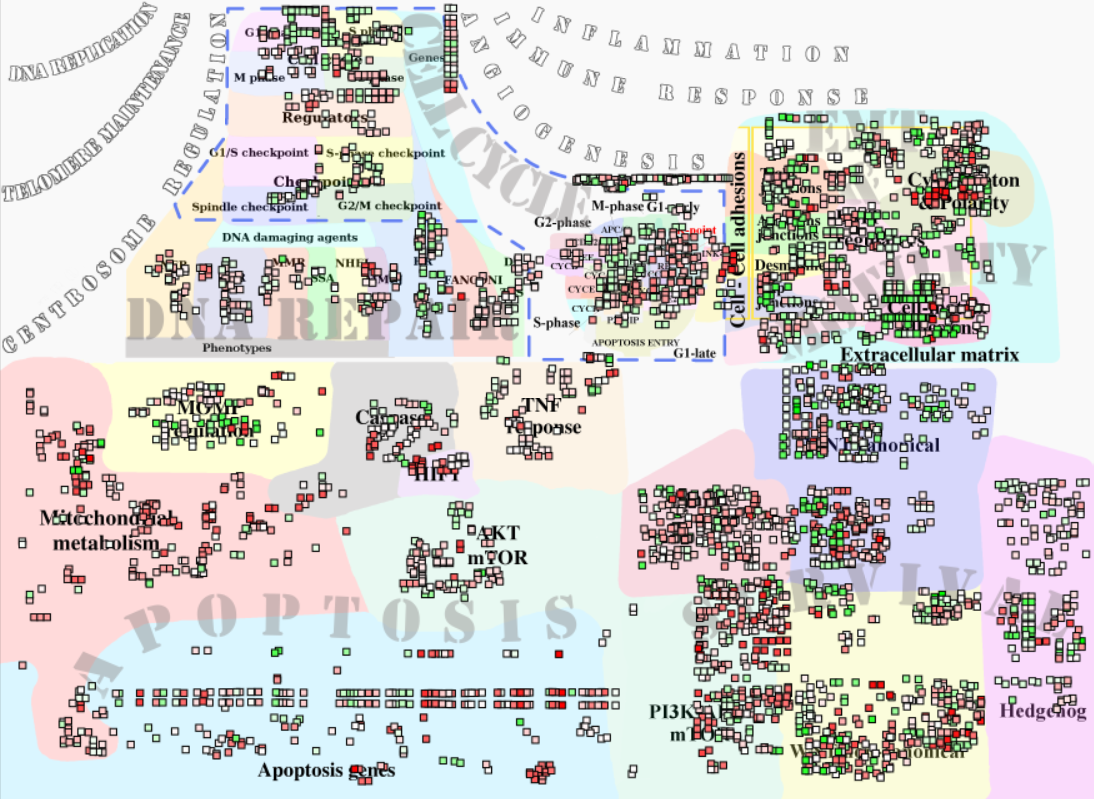
\includegraphics[width=0.8\textwidth]{figures/mainz_acsn.png}
  \label{fig:mainz}
\end{figure}

\subsection{Analysis of glioblastoma mutation frequencies}

Recent years have witnessed a dramatic increase in new technologies for
interrogating the activity levels of various cellular components on a
genome-wide scale, including genomic, epigenomic, transcriptomic, and proteomic
information \citep{hawkins2010next}. Integrating these heterogeneous datasets
provides more biological insights than performing separate analyses. For
instance, international consortia such as The Cancer Genome Atlas (TCGA) have
launched large-scale initiatives to characterize multiple types of cancer at
different levels on hundreds of samples.  These integrative studies have
already led to the identification of novel cancer genes
\citep{mclendon2008comprehensive}. 

Malignant gliomas, the most common subtype of primary brain tumors, are
aggressive, highly invasive, and neurologically destructive tumors considered
to be among the deadliest of human cancers. In its most aggressive
manifestation, glioblastoma (GBM), median survival ranges from 9 to 12 months,
despite maximum treatment efforts \citep{maher2001malignant}. In this study we
have analyzed whole-genome mutation data generated by the TCGA project on
hundreds of patients. More specifically, we parsed the MAF (Mutation Annotation
Format) GBM files produced by different sequencing centers to count and
calculate gene mutation frequencies. We kept the mutations having a status
likely to disturb the target protein's function (i.e, Frame\_Shift\_Del,
Nonstop\_Mutation, In\_Frame\_Del, In\_Frame\_Ins, Missense\_Mutation,
Nonsense\_Mutation, Splice\_Site, Translation\_Start\_Site). In total, we
collected mutations for more than 13,000 genes in a total of 379 mutated
samples. In order to retain the most frequently mutated genes, we calculated
frequencies across all mutated samples, and kept genes having a frequency
greater than 1\% (3,293 genes). We further labelled genes having a frequency
greater than 1\% and less than 5\% as "1" and genes highly mutated (frequency
higher than 5\%) as "2". 

We loaded the data as a matrix in R and calculated the enrichment in ACSN maps
with the ACSNMineR function \code{enrichment}. The results are displayed in
table \ref{tab:table_gbm}. There are 6 modules significantly enriched in the
DNA repair and EMT motility maps. Cell matrix adhesions and ECM
(extra cellular matrix), part of the EMT motility map, are the modules with
highest significance. The EMT motility map is significantly enriched at the
global map level (second line in the table). 

\begin{table}[h!]
  \centering
  \caption{ACSN maps enrichment for frequently mutated glioblastoma genes.
  Module : name of the module. Mod. size: size of the module. Nb genes: number
  of genes from input which are found in the module. Cor. pval: corrected
  p-value.} 
  \label{tab:table_gbm}

\begin{tabular}{l c c c}
\toprule
module & Mod. size & Nb genes & Cor. pval\\ 
\midrule
DNA\_repair:S\_PHASE\_CHECKPOINT &   45 &      19 &     0.008\\
EMT\_motility  &  635  &   181  &   0.0002\\
EMT\_motility:CELL\_MATRIX\_ADHESIONS   &   73  &    45  &    3.73e-12\\
EMT\_motility:CYTOSKELETON\_POLARITY   &   154 &    47  &    0.022\\
EMT\_motility:DESMOSOMES & 29  &    15  &    0.002\\
EMT\_motility:ECM    &    147  &   69   &   9.77e-11\\
EMT\_motility:EMT\_REGULATORS  &   629   &  178  &   0.0002\\
\bottomrule
\end{tabular}
\end{table}

Visualization of the list of glioblastoma mutated genes is shown on figure
\ref{fig:gbm}. This figure was generated with the ACSNMineR commands detailed
below. Results of the enrichment test correlate well with the visualization on
the map, with a high density of low and high frequency mutated genes in the EMT
motility and DNA repair regions (maps) of the global ACSN map. Although they
are not statistically significant, quite high densities can also be seen in
other regions of the map.

\begin{example}
library(RNaviCell)

# Create a NaviCell object, point it to the ACSN master map and launch
# a session.

navicell <- NaviCell()
navicell$proxy_url <- "https://acsn.curie.fr/cgi-bin/nv_proxy.php"
navicell$map_url <- "https://acsn.curie.fr/navicell/maps/acsn/master/index.php"
navicell$launchBrowser()

# Read the GBM data file and import it into the session.

mat <- navicell$readDatatable('gbm.txt')
navicell$importDatatable("Mutation data", "GBM", mat)

# set datatable and sample names for the glyph editor

navicell$drawingConfigSelectGlyph(1, TRUE)
navicell$glyphEditorSelectSample(1, "categ")
navicell$glyphEditorSelectShapeDatatable(1, "GBM")
navicell$glyphEditorSelectColorDatatable(1, "GBM")
navicell$glyphEditorSelectSizeDatatable(1, "GBM")
navicell$glyphEditorApply(1)

# set color, shape and size parameters for glyphs

navicell$unorderedConfigSetDiscreteShape("GBM", "sample", 0, 1)
navicell$unorderedConfigSetDiscreteShape("GBM", "sample", 1, 5)
navicell$unorderedConfigApply("GBM", "shape")

navicell$unorderedConfigSetDiscreteColor("GBM", "sample", 0, "398BC3")
navicell$unorderedConfigSetDiscreteColor("GBM", "sample", 1, "CC5746")
navicell$unorderedConfigApply("GBM", "color")

navicell$unorderedConfigSetDiscreteSize("GBM", "sample", 0, 4)
navicell$unorderedConfigSetDiscreteSize("GBM", "sample", 1, 14)

navicell$unorderedConfigApply("GBM", "size")
\end{example}


\begin{figure}[!ht]
  \caption{Glioblastoma gene mutation frequency categories represented as
  glyphs on the ACSN global cancer map. High frequency mutated genes are
  pictured as large red circles, while low frequency mutated genes are depicted
  as small blue squares.
  } 
  \centering
  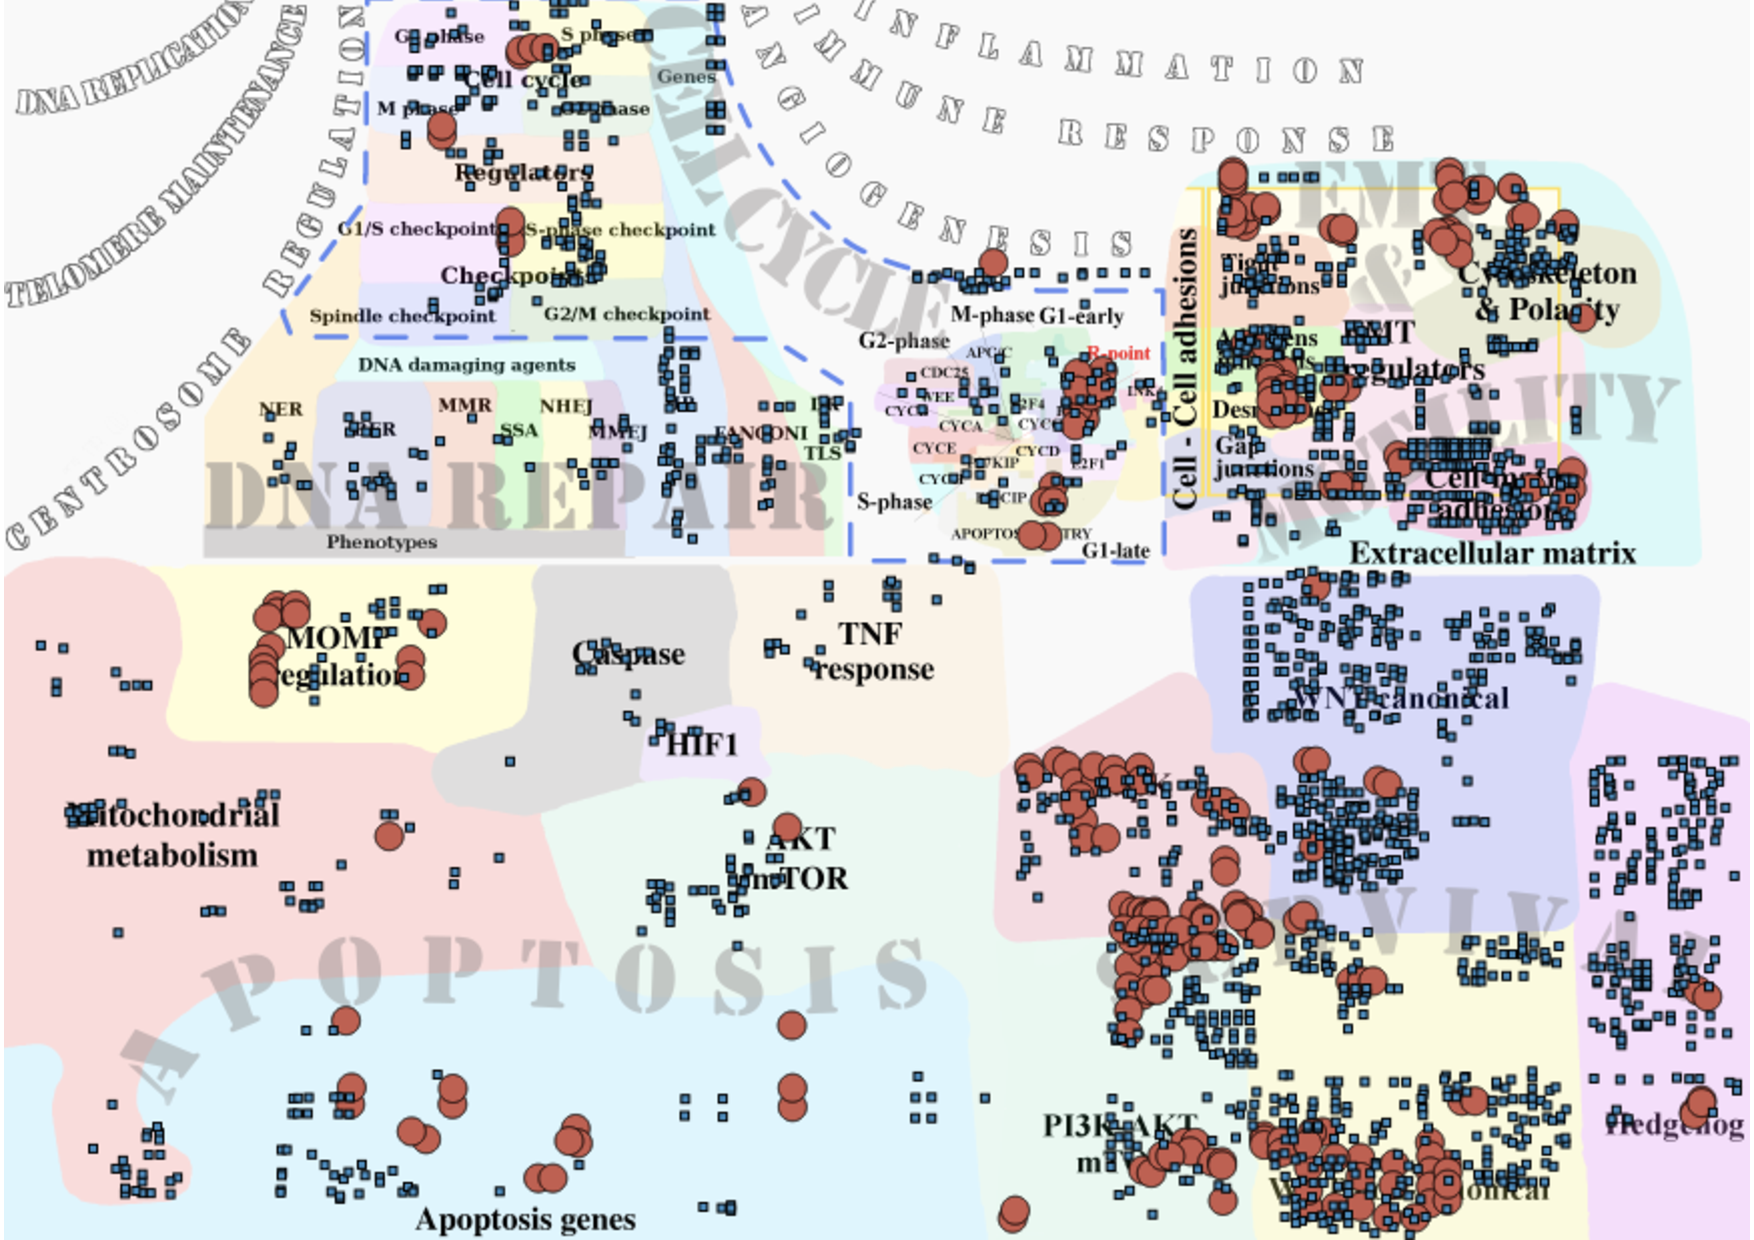
\includegraphics[width=0.8\textwidth]{figures/gbm.pdf}
  \label{fig:gbm}
\end{figure}

\section[Summary and perspectives]{Summary and perspectives}

In this work, we presented the R package \pkg{ACSNMineR}, a novel package for
the calculation of p-values for enrichment or depletion of genes in biological
pathways. The package includes the six large-scale molecular maps and 55
functional modules of the Atlas of Cancer Signaling Network (ACSN) . Enrichment
can be calculated for those maps and modules with several options to play with,
but can also be calculated for other databases of molecular pathways, that can
be imported from GMT formated files. 

We also describe in this work the \pkg{RNaviCell} package, a R package
convenient to use with \pkg{ACSNMineR}. This package is dedicated to create
web-based and interactive data visualization on ACSN maps. Users can use this
tools to represent genes of interest that have been shown to be related to the
maps by calculating enrichment with the  \pkg{ACSNMineR}.  Creating maps with
the graphical user interface of the ACSN website can be a tedious task if the
user has multiple samples or gene lists, and wants to compare their
representations on ACSN maps. The \pkg{RNaviCell} package can be used to
automate the process of creating the graphical representations automatically. 

We have shown how the packages \pkg{ACSNMineR} and \pkg{RNaviCell} can be
combined to analyze expression data from breast cancer samples, and also to
analyze the frequency of mutated genes in glioblastoma cancer samples.  

Of course, \pkg{ACSNMineR} is not the only R package for enrichment
calculations. For instance, \BIOpkg{GOstats} \citep{falcon2007using} is
probably one of the first packages that was created to calculate enrichment for
Gene Ontology categories.  \pkg{GOstats} can also be used to calculate
enrichment for other biological pathways categories, such as KEGG pathways (by
using an instance of the class \code{KEGGHyperGParams}) or PFAM protein
families (using \code{PFAMHyperGParams}). However, its usage might not be as
straightforward as \pkg{ACSNMineR}, and it does not seem possible to test
user-defined biological pathways. Furthermore, other authors have pointed out
that the KEGG database used by this package has not been updated since 2012.
\BIOpkg{clusterProfiler} is a recent R package released for enrichment analysis
of Gene Ontology and KEGG with either hypergeometric test or Gene Set
Enrichment Analysis (GSEA) \citep{yu2012clusterprofiler}. Via other packages,
support for analysis of Disease Ontology and Reactome Pathways is possible.
Interestingly, this package also offers the possibility to import user-defined
gene set, through tab-delimited pairwise definition files. Other notable
packages for enrichment calculations are \pkg{ReactomePA} for Reactome molecular
pathways \citep{ReactomePA2016}, \pkg{miRNApath} for microRNA pathways
\citep{miRNApath2008} and \pkg{gage} \citep{gage2009}. We believe that the main
advantages of ACSNMineR compared to other packages are a direct access to the
full set of ACSN maps (updated on a regular basis) and an easy way to test
MSigDB gene sets or any user-defined gene set formatted appropriately.

In order to improve \pkg{ACSNMineR}, we may in the near future try to improve
the speed of calculation, which might be a problem if a very large number of
samples or experiments have to be analyzed rapidly. For instance, we could use
the \code{foreach} and \code{\%dopar\%} operator to parallelize the most
computationally demanding operations. It could also be useful to implement more
sensitive methods of gene set enrichment measures, such as the Gene Set
Enrichment Analysis (GSEA) method. 

\pkg{RNaviCell} relies on standard HTTP calls to provide informations and
calculations, and we have developped a number of bindings for popular
programming languages such as R, Java and Python \citep{bonnet2015navicell}.
This open architecture is designed to facilitate the development of utilities
by other programmers and to facilitate the integration of ACSN maps in existing
frameworks. The development of such services, sometimes called ``microservices"
\citep{fowler2014} is in expansion. Furthermore, this kind of open architecture
could clear the way for a more unified and general access to reaction networks
database, including for example WikiPathways \citep{kelder2012wikipathways},
Reactome \citep{croft2014reactome} and other databases. The PSICQUIC project is
a successfull example of such an architecture \citep{aranda2011psicquic}. It is
an effort of the HUPO proteomics standard initiative to standardize the access
to molecular interaction databases programmatically, based on the specification
of web services (using REST and SOAP calls) and a common query language (MIQL).

\section[Acknowledgments]{Acknowledgements}

This work was supported by a grant ``Projet Incitatif et Collaboratif
Computational Systems Biology Approach for Cancer" from Institut Curie. The
authors would like to thank Pierre Gestraud for his comments on early versions
of the \pkg{ACSNMineR} package and Eric Viara for guidance and assistance on
the development of the \pkg{RNaviCell} package.


\bibliography{Deveau}

\address{
  Paul Deveau\\
  Computational Systems Biology of Cancer, Institut Curie\\
  26, rue d'Ulm 75248 Paris\\
  France\\
}
\email{paul.deveau@curie.fr}

\address{
  Emmanuel Barillot\\
  Computational Systems Biology of Cancer, Institut Curie\\
  26, rue d'Ulm 75248 Paris\\
  France\\
}
\email{emmanuel.barillot@curie.fr}

\address{
  Valentina Boeva\\
  Computational Systems Biology of Cancer, Institut Curie\\
  26, rue d'Ulm 75248 Paris\\
  France\\
}
\email{valentina.boeva@curie.fr}

\address{
  Andrei Zinovyev\\
  Computational Systems Biology of Cancer, Institut Curie\\
  26, rue d'Ulm 75248 Paris\\
  France\\
}
\email{andrei.zinovyev@curie.fr}

\address{
  Eric Bonnet\\
  Centre National de Génotypage, Institut de Génomique, CEA\\
  2, rue Gaston Crémieux, 91057 Evry\\
  France\\
}
\email{eric.bonnet@cng.fr}
